\section{Visualisation tools in ML4PG}\label{sec:visualisation}


In the previous section, we have seen how ML4PG can be used to find families of proofs following
a common proof pattern. However, the output provided by clustering algorithms is just a set
of similar patches with no hints of why these proof-patches are deemed similar.
In this section, we present our approach to facilitate the understanding of proof patterns.


The first problem that we address is the discovery of the key features that were taken
into account during the cluster formation. This is a well-known problem in machine-learning
known as \emph{feature selection}~\cite{Weka}. From a given set of features, feature selection algorithms
generate different subsets of features and create a ranking of feature subsets.
ML4PG uses the \emph{correlation-based feature subset selection} algorithm implemented in Weka~\cite{Weka}
-- the machine-learning toolbox employed by ML4PG to extract the relevant features.

\begin{example}\label{ex:correlation-features}
In the case study presented at the end of the previous section, the relevant features were:

$-$ The tactics applied in the first and second steps of the proof-patches (\lstinline?case? and \lstinline?rewrite? respectively).

$-$ The type of the argument of the tactic applied in the first step of the proof-patches (\lstinline?nat?).

$-$ The second top symbol of the goal in the second step of the proof-patches (the $\sum$ symbol).

$-$ The first and second auxiliary lemmas applied in the the third step of the proof-patches. The first auxiliary lemma (\lstinline?sumrB?) is used to expand the summations and is
common to all the proofs. There are two different \lq\lq{}second\rq\rq{} auxiliary lemmas that occur in the proofs of Lemma~\ref{lem:fundamental} and~\ref{lem:nilpotent2} (\lstinline?big_nat_recr? and
\lstinline?big_nat_recl? -- both extract elements of a summation); however, the recurrent feature extraction process have assigned similar values to them.
The ``automaton'' of Example~\ref{ex:correlation-features} is depicted in Figure~\ref{fig:automata} and Appendix~\ref{sec:automaton}.
\end{example}

ML4PG uses this information and produces an automaton-shape representation for discovered
proof-patterns and the correlated features that determined the patterns.
Our graphical representation is simpler than other works where automata are used to represent models that are inferred from proof traces~\cite{GWR14}.

Generally, given a cluster of proof patches ${\cal C}$, we have an automaton $A$ with $5$ consecutive states. The $i$th state of $A$ is labelled
with the list of $i$th goals in the proof-patches contained in ${\cal C}$. The transitions between the $i$th and $i+1$th states are given by
the $i$th tactic of each proof-patch of ${\cal C}$. If two or more tactics belong to the same group (see Figure~\ref{tab:tactics}),
they are merged in a unique transition; otherwise, the tactics will be shown as different transitions. In addition, each state is annotated with
features
whose correlation determined the cluster.


\begin{figure}[t]
\centering
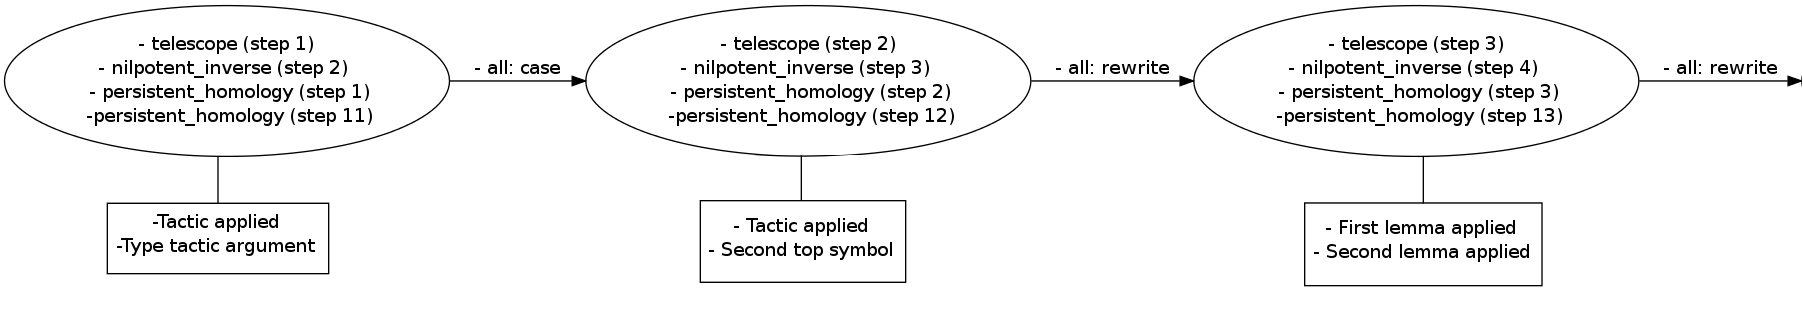
\includegraphics[scale=.19]{itp6.png}
\caption{\scriptsize{\emph{Fragment of the automaton
 corresponding to the cluster of four lemma fragments described in the case study of Section~\ref{sec:recurrent}} (the whole automaton can be seen in Appendix~\ref{sec:automaton}).
It shows correspondence between certain proof steps of lemmas
\texttt{telescope} (for the lemma of Example~\ref{example0}), \texttt{nilpotent\_inverse} (for Lemma~\ref{lem:nilpotent2}), and \texttt{persistent\_homology}
(for Lemma~\ref{lem:fundamental}). Square boxes denote feature correlation where it exists.
To be compact, we  hide full lemma statements, tactic and auxiliary lemma names, symbols, etc., but they can be shown by ML4PG.

}}\label{fig:automata}
\end{figure}
